\documentclass[10pt,twocolumn,letterpaper]{article}

% ---------- CVPR-style layout ----------
\usepackage[top=1in,bottom=1in,left=0.75in,right=0.75in,columnsep=0.25in]{geometry}
\usepackage{times}
\usepackage{graphicx}
\usepackage{amsmath,amssymb}
\usepackage{booktabs}
\usepackage{microtype}
\usepackage{caption}
\usepackage{subcaption}
\usepackage{float}
\usepackage{enumitem}
\usepackage{xcolor}
\usepackage[hidelinks,colorlinks=true,linkcolor=black,citecolor=black,urlcolor=blue]{hyperref}
\usepackage{titlesec}
\usepackage{abstract}

% Section heading style (mimicking CVPR)
\titleformat{\section}{\normalfont\large\bfseries}{\thesection}{1em}{}
\titleformat{\subsection}{\normalfont\normalsize\bfseries}{\thesubsection}{1em}{}
\titleformat{\subsubsection}{\normalfont\normalsize\itshape}{\thesubsubsection}{1em}{}
\titlespacing*{\section}{0pt}{8pt plus 2pt minus 2pt}{4pt plus 1pt}
\titlespacing*{\subsection}{0pt}{6pt plus 2pt minus 2pt}{3pt plus 1pt}

% Abstract style (single-column title + abstract, then two-column body)
\renewenvironment{abstract}
  {\small\quotation\noindent\textbf{Abstract.}\enspace}
  {\endquotation}

% Caption style
\captionsetup{font=small,labelfont=bf,skip=4pt}

% Remove paragraph indent, add small skip
\setlength{\parindent}{0pt}
\setlength{\parskip}{4pt}

% References (manual thebibliography, no bibtex needed)

% -----------------------------------------------
\begin{document}

% ===== TITLE BLOCK (one-column) =================
\twocolumn[{%
\begin{center}
  {\LARGE\bfseries Explaining GPT-2 with AttnLRP: Token Attribution,\\[2pt]
  Fine-Tuning Effects, and Parameter-Level Analysis}\\[10pt]
  {\large Yenchi Tseng \quad Fangteng Fu}\\[4pt]
  {\normalsize The Hong Kong University of Science and Technology (Guangzhou)}\\[4pt]
  {\normalsize AIAA 4051 Natural Language Processing — Final Project, 2025}\\[14pt]
\end{center}
\begin{abstract}
Understanding how transformer-based language models allocate internal
relevance to inputs is a central challenge in explainable AI.
This paper applies \textbf{AttnLRP}~\cite{achtibat2024attnlrp}, specifically
its \emph{CP-LRP} variant, to \textbf{GPT-2 Small} across three complementary
levels of analysis.
\textbf{Task~1} implements token-level attribution on the SQuAD\_v2 validation
set (200 samples) and evaluates faithfulness via a Pixel Flipping protocol.
CP-LRP reliably highlights named entities and question keywords, and achieves a
lower normalised AUC than a random baseline (0.0190 vs.\ 0.0490), confirming
faithfulness. Its dual-signed scores also produce a non-monotonic deletion curve,
motivating polarity-aware evaluation metrics.
\textbf{Task~2} compares CP-LRP attributions before and after sequential
fine-tuning on SQuAD\_v2 followed by SciQ, showing that task-specific training
systematically shifts relevance toward question-side tokens and answer-relevant
entities.
\textbf{Task~3} extends attribution to the parameter level, comparing two
models fine-tuned independently on SciQ and SQuAD\_v2 using 1{,}000 evaluation
inputs each (SciQ test split; SQuAD\_v2 validation split), and finds that the SciQ-finetuned model engages upper MLP layers
(Layers~9 and~10) more strongly ($\Delta = +0.0196$ at Layer~10), while the
SQuAD\_v2-finetuned model shows higher engagement at middle layers
($\Delta = -0.0126$ at Layer~6),
consistent with the different roles of parametric memory versus in-context
retrieval in the two tasks.
Together, these experiments demonstrate AttnLRP as a practical tool for
auditing attribution patterns at the token, fine-tuning, and parameter levels.
\end{abstract}
\vspace{10pt}
}]

% ===== SECTION 1: INTRODUCTION =================
\section{Introduction}
\label{sec:intro}

Large language models (LLMs) based on the transformer architecture have
achieved strong empirical performance on a wide range of natural language tasks.
Yet the internal mechanisms by which these models arrive at their predictions
remain difficult to interpret.
Explainability techniques that assign importance scores to individual inputs
are therefore an active area of research, with practical implications for model
debugging, trust calibration, and regulatory compliance.

Layer-wise Relevance Propagation (LRP)~\cite{bach2015pixel} is a principled
attribution framework that decomposes a model's scalar output into additive
contributions from each input feature by back-propagating relevance through
the network according to conservation rules.
Applying LRP to transformers, however, requires care: the attention softmax
introduces a non-linear routing operation that standard LRP rules do not handle
correctly, and na\"ive gradient-based attributions through attention weights can
produce noisy or misleading scores.

\textbf{AttnLRP}~\cite{achtibat2024attnlrp} addresses this by introducing
modified LRP rules tailored to the attention mechanism.
Its \emph{CP-LRP} variant, recommended for models with potentially negative
logits such as GPT-2, stops gradient flow through the query and key branches
of the attention softmax while preserving it through the value pathway.
This produces token-level relevance scores with clear positive/negative
semantics: a positive score indicates that the token promotes the predicted
output, while a negative score indicates suppression.

Question answering (QA) provides a particularly informative setting for
attribution analysis.
A QA prompt has a structured format comprising a question, an
optional supporting context, and an answer boundary, which together create clear
semantic segments whose differential relevance can be measured and
interpreted.
When a context passage is present, named entities and answer-bearing spans
have unambiguous semantic roles, making qualitative validation of attribution
heatmaps straightforward.
At the same time, the causal chain from input tokens to the predicted answer
token is complex enough to stress-test attribution methods: the model must
jointly process long-range contextual information and query-side intent before
committing to a single output.
This structure makes QA ideal for evaluating whether an attribution method
captures semantically meaningful, task-relevant signal.

In this project we apply CP-LRP to \textbf{GPT-2 Small}~\cite{radford2019gpt2}
(124M parameters, 12 transformer blocks, hidden size 768) and investigate three
complementary questions:
\begin{enumerate}[leftmargin=*, itemsep=0pt, topsep=2pt]
  \item Can CP-LRP reliably identify semantically meaningful tokens in a
        question-answering context, and do its attributions pass a quantitative
        faithfulness test?
  \item How does sequential fine-tuning on two QA datasets change the token
        relevance distribution?
  \item Do models fine-tuned on different tasks exhibit measurable differences
        in how they allocate relevance across transformer layers at the
        parameter level?
\end{enumerate}

% ===== SECTION 2: RELATED WORK =================
\section{Related Work}
\label{sec:related}

\paragraph{Layer-wise Relevance Propagation.}
LRP was introduced by Bach et al.~\cite{bach2015pixel} as a method for
explaining the decisions of deep neural networks by redistributing the output
score back to the input pixels according to relevance conservation rules.
Various propagation rules (LRP-$\varepsilon$, LRP-$\gamma$, etc.) have since
been proposed to handle different layer types and improve attribution quality.

\paragraph{AttnLRP.}
Achtibat et al.~\cite{achtibat2024attnlrp} derived attention-aware LRP rules
for transformer architectures and showed that na\"ive application of standard
LRP to attention layers produces attributions inconsistent with model
computations.
CP-LRP specifically addresses models where logits can be negative by applying a
\emph{stop-gradient} operation on the query and key tensors before the
attention softmax, ensuring that relevance is propagated only through the
value-weighted path.

\paragraph{Faithfulness evaluation.}
Samek et al.~\cite{samek2017evaluating} proposed the Pixel Flipping (also
called token deletion or ROAR) paradigm as a model-agnostic faithfulness
metric: tokens are masked in decreasing order of attributed importance, and a
faithful explanation should cause confidence to drop faster than a random
baseline.
The standard protocol sorts tokens by absolute attribution magnitude; when
signed attributions are instead sorted by their signed value (most positive
first), masking eventually crosses into the negatively-relevant region and
can produce non-monotonic confidence curves.
We discuss this behaviour and its implications for evaluation in
Section~\ref{sec:task1}.

\paragraph{Attention weights as explanations.}
A natural but unreliable alternative to propagation-based attribution is to
use raw attention weights as a proxy for token importance.
Jain and Wallace~\cite{jain2019attention} demonstrated that attention weights
are weakly correlated with gradient-based feature importance measures and can
be arbitrarily manipulated without changing model predictions, casting doubt
on their use as faithful explanations.
Wiegreffe and Pinter~\cite{wiegreffe2019attention} further showed that
alternative attention distributions can produce identical predictions,
confirming that attention alone does not constitute a sufficient explanation.
These findings motivate the use of a principled back-propagation framework
such as AttnLRP, which distributes relevance through the full computational
graph rather than reading off intermediate attention coefficients.

% ===== SECTION 3: METHODOLOGY =================
\section{Methodology}
\label{sec:method}

\subsection{CP-LRP Implementation}

We implement CP-LRP using the \texttt{lxt} (LRP-eXplains-Transformers) library
with manual compatibility patches for Hugging Face \texttt{transformers}
v4.44.2.
Three types of modifications are applied to GPT-2 Small before loading model
weights:

\begin{itemize}[leftmargin=*, itemsep=0pt, topsep=2pt]
  \item \textbf{Attention (CP-LRP rule):} The internal \texttt{\_attn} method
        of \texttt{GPT2Attention} is patched to wrap the query and key tensors
        with \texttt{stop\_gradient} before passing them to the attention
        softmax.
        Relevance therefore flows only through the value pathway.
  \item \textbf{MLP blocks:} The \texttt{GPT2MLP.forward} method is replaced
        with the LXT identity-rule forward pass, which propagates relevance
        without modifying the activation denominator.
  \item \textbf{LayerNorm and Dropout:} Both are patched with identity-rule
        forwards, treating them as pass-through operations for relevance
        purposes.
\end{itemize}

Token-level relevance scores are obtained via the gradient$\times$input
formula applied at the embedding layer:

\begin{equation}
  R_i = \sum_{d=1}^{D} e_{i,d} \cdot \frac{\partial \hat{y}}{\partial e_{i,d}},
  \label{eq:relevance}
\end{equation}

where $e_i \in \mathbb{R}^D$ is the embedding of the $i$-th input token,
$D = 768$ is the embedding dimension, and $\hat{y}$ is the maximum logit at
the final sequence position.
Each score $R_i$ is a signed scalar: positive values promote and negative
values suppress the predicted next token.

\subsection{Parameter-Level Relevance (Task~3)}

To compare how different fine-tuning domains engage each transformer block, we
extend the attribution to the MLP weight matrices.
For each block $\ell$, we compute:

\begin{multline}
    R_\ell^{\mathrm{param}}
      = \sum_{i,j}
        \left| W_{ij}^{(c\_fc,\ell)} \cdot
               \frac{\partial \hat{y}}{\partial W_{ij}^{(c\_fc,\ell)}} \right|
  \\
      + \sum_{i,j}
        \left| W_{ij}^{(c\_proj,\ell)} \cdot
               \frac{\partial \hat{y}}{\partial W_{ij}^{(c\_proj,\ell)}}
  \right|,
    \label{eq:param-relevance}
\end{multline}

where $W^{(c\_fc,\ell)} \in \mathbb{R}^{768 \times 3072}$ and
$W^{(c\_proj,\ell)} \in \mathbb{R}^{3072 \times 768}$ are the two linear
projection weights of the feed-forward network in block $\ell$.
Gradients are enabled only for MLP parameters; the CP-LRP patches remain
active so that backward passes follow the same propagation rules.
Scores are averaged over all evaluation inputs and then normalised by the total
relevance sum across all 12 layers.

% ===== SECTION 4: TASK 1 =================
\section{Task 1: Token Attribution on SQuAD\_v2}
\label{sec:task1}

\subsection{Experimental Setup}

We take the first 200 examples from the SQuAD\_v2 validation split.
Each example is formatted as a causal language modelling prompt:

\vspace{3pt}
\texttt{Context: <context[:300]>}\\
\texttt{Question: <question>}\\
\texttt{Answer:}
\vspace{3pt}

The pretrained GPT-2 Small (no fine-tuning) is used as the analysis target.
CP-LRP relevance is computed for every token via Equation~\eqref{eq:relevance},
and 200 per-sample heatmaps are rendered with a diverging RdYlGn colormap
(green = positive, red = negative).

\subsection{Qualitative Results}

Figure~\ref{fig:heatmap} shows a representative token heatmap.
Three recurring patterns appear consistently across the 200 samples:

\textbf{Named entities and content words receive the highest positive
relevance.}
In examples asking about geographic locations or persons, the relevant noun
phrases in both the context and the question are highlighted in green,
indicating that the model correctly identifies them as the most predictive
features for next-token generation.

\textbf{The \texttt{Answer:} delimiter token is strongly negative.}
This structural token marks the boundary between prompt and generation; its
suppressive relevance score reflects that masking it would dramatically shift
the input distribution away from the question-answering regime.

\textbf{Function words and punctuation are near-neutral.}
Articles, prepositions, and commas consistently receive relevance scores close
to zero, consistent with their low semantic specificity.

\begin{figure}[t]
  \centering
  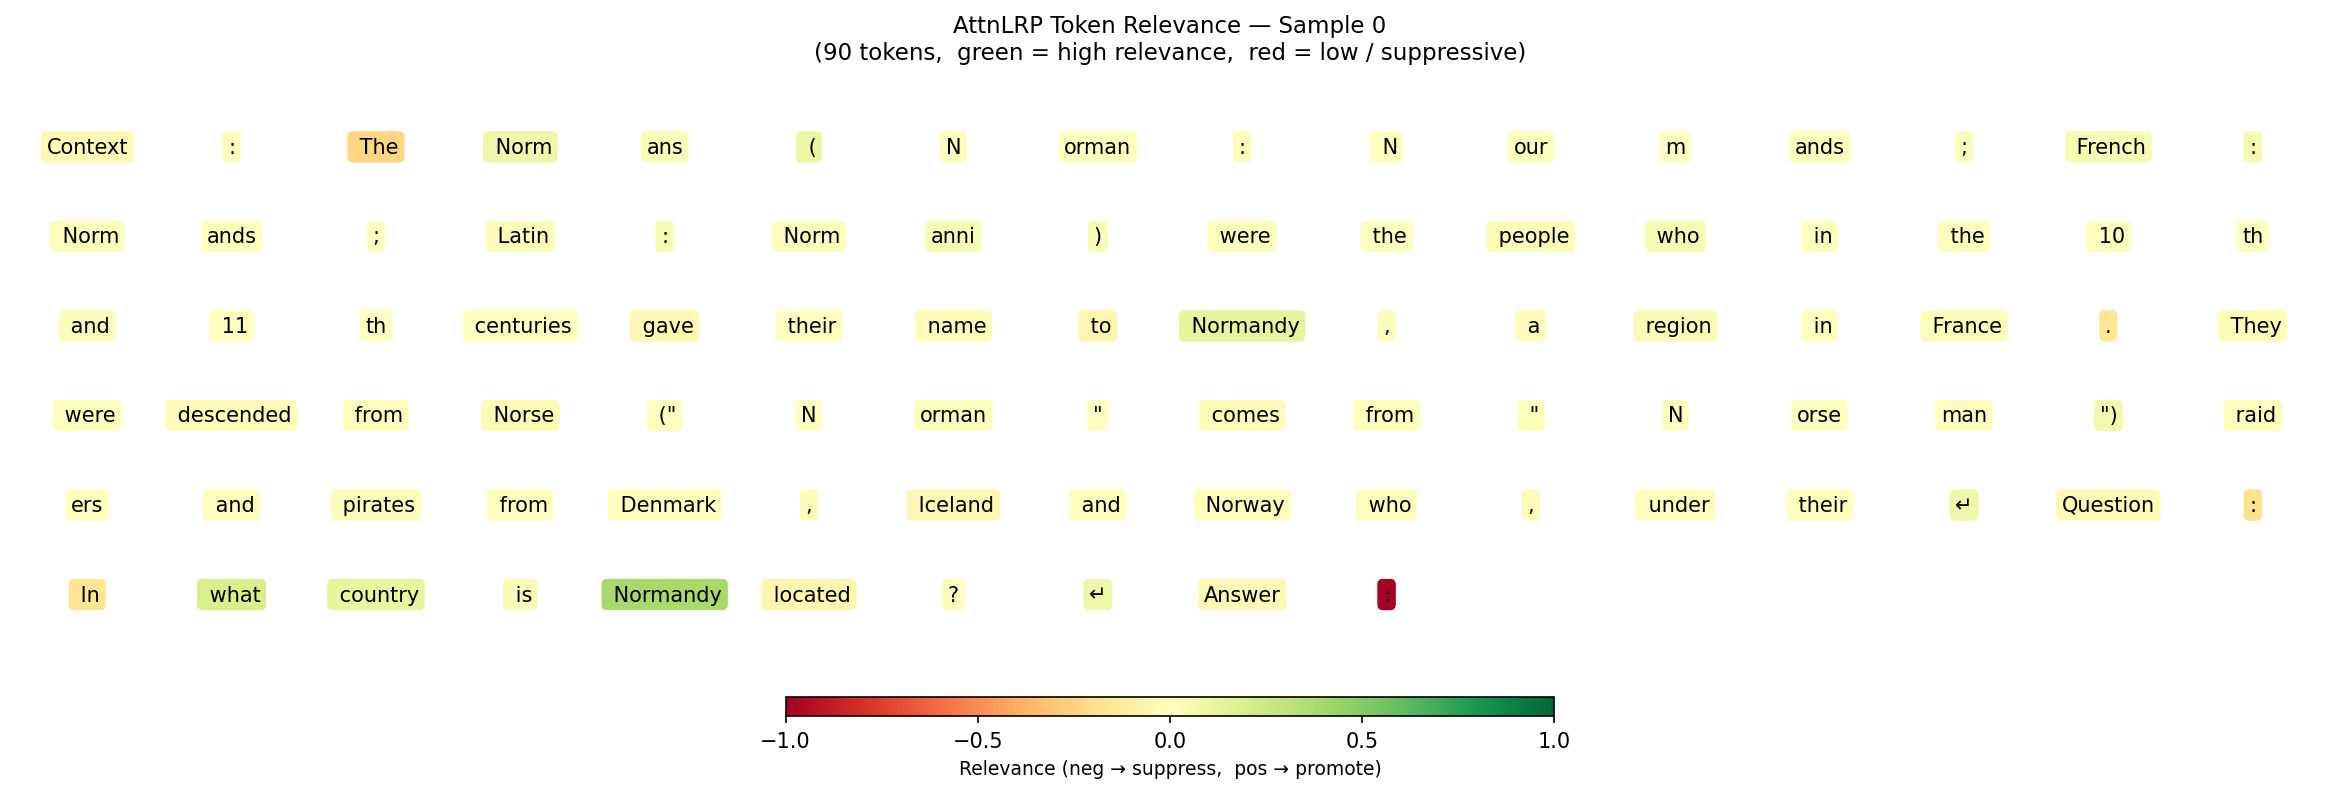
\includegraphics[width=\linewidth]{aiaa4051/task1/relevance/sample_0.png}
  \caption{CP-LRP token relevance heatmap for a representative SQuAD\_v2 sample
    (``In what country is Normandy located?'').
    Green = positive (promotes prediction); red = negative (suppresses).
    Named entities (\texttt{Normandy}) receive the highest positive relevance;
    the \texttt{Answer:} delimiter is strongly negative.}
  \label{fig:heatmap}
\end{figure}

\subsection{Faithfulness Evaluation}
\label{sec:faithfulness}

We evaluate whether the relevance ranking is faithful to the model's
computation using a \textbf{Pixel Flipping} protocol~\cite{samek2017evaluating}.
Tokens are progressively masked (via \texttt{attention\_mask = 0}, leaving
token ids unchanged) in three orderings:
\begin{enumerate}[leftmargin=*, itemsep=0pt, topsep=2pt]
  \item \textbf{AttnLRP order}: descending signed relevance (most positive first).
  \item \textbf{Random order}: random permutation (seed 42, averaged over 200
        samples).
  \item \textbf{Least-relevant-first}: ascending absolute relevance.
\end{enumerate}
At each masking step the model's confidence in its original prediction (the
softmax probability of the initially predicted next token) is recorded.
Results are averaged across all 200 samples.
Table~\ref{tab:auc} reports normalised AUC scores (integral of the mean
confidence curve divided by 100\%).

\begin{table}[h]
  \centering
  \small
  \begin{tabular}{lc}
    \toprule
    \textbf{Deletion order} & \textbf{Normalised AUC} \\
    \midrule
    AttnLRP (most relevant first) & 0.0190 \\
    Random baseline               & 0.0490 \\
    Least-relevant-first (baseline) & 0.0871 \\
    \bottomrule
  \end{tabular}
  \caption{Pixel Flipping normalised AUC (200 SQuAD\_v2 samples). Lower AUC
    indicates faster confidence decay. Least-relevant-first provides an upper bound on AUC (worst-case deletion order, slowest confidence decay).}
  \label{tab:auc}
\end{table}

\begin{figure}[t]
  \centering
  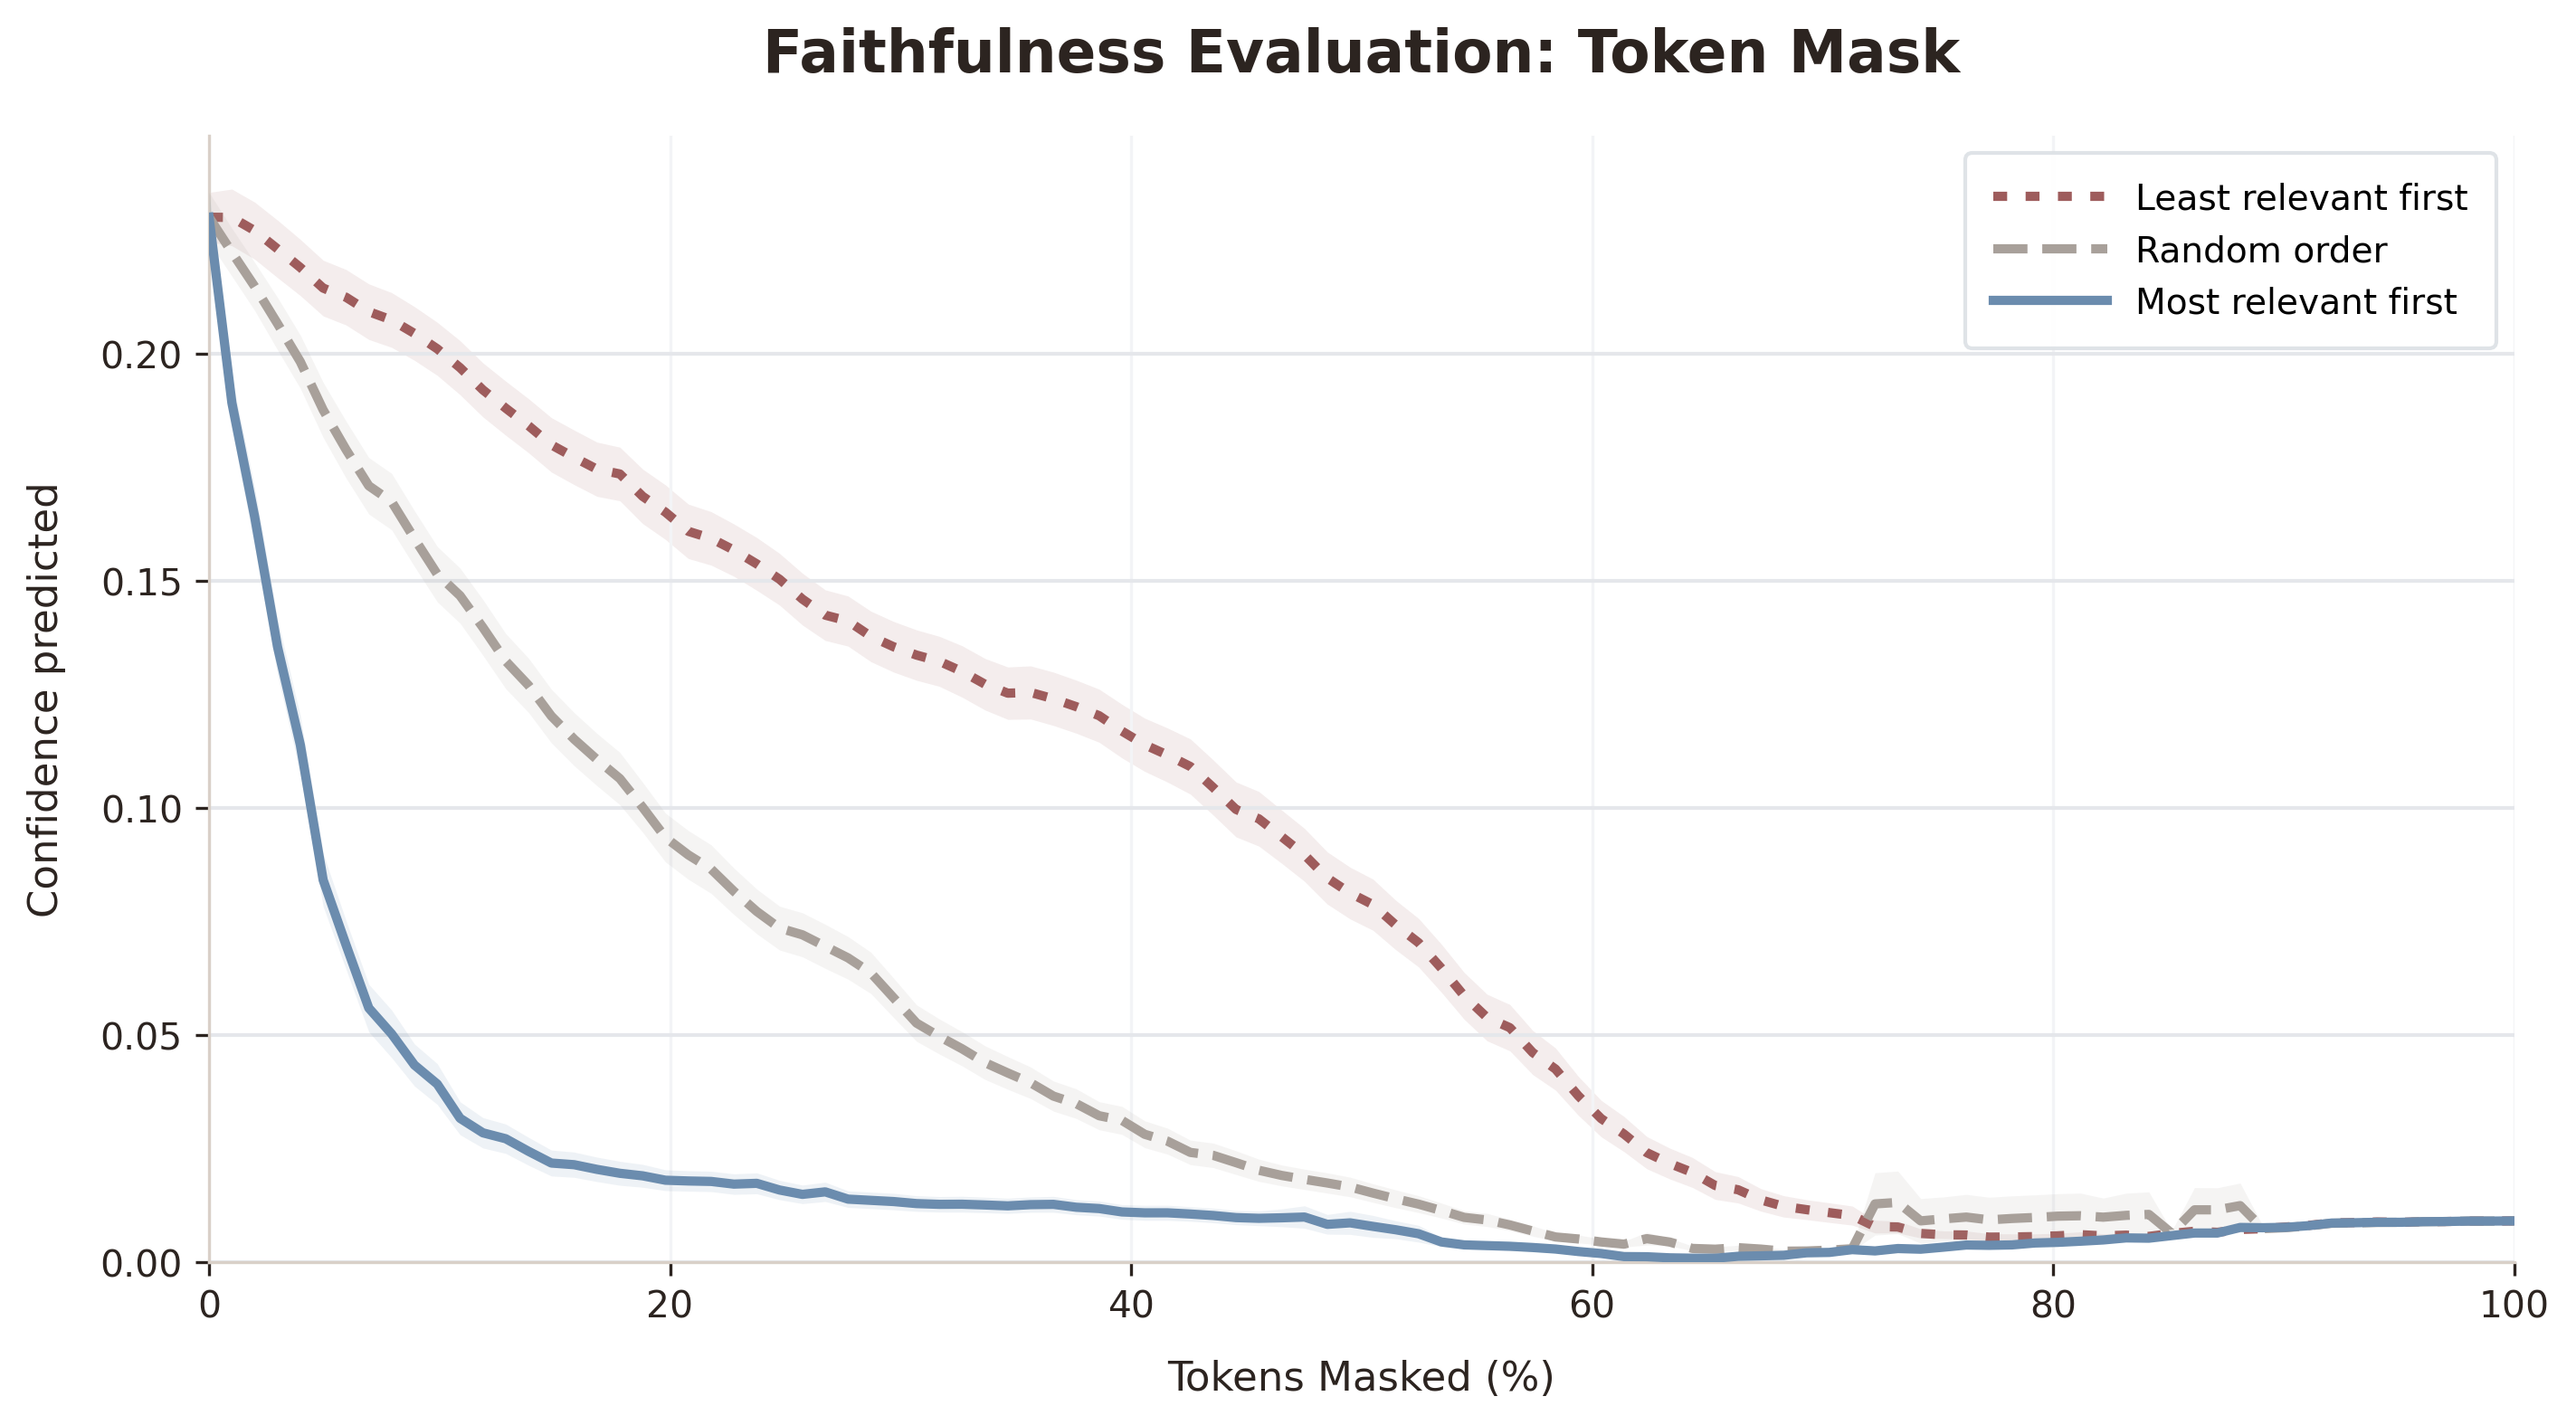
\includegraphics[width=\linewidth]{aiaa4051/task1/faithfulness/faithfulness_curve.png}
  \caption{Pixel Flipping confidence curves averaged over 200 samples.
    The AttnLRP curve (blue) exhibits a characteristic non-monotonic shape:
    confidence initially declines as positively-relevant tokens are masked,
    then rises when masking transitions into negatively-relevant (suppressive)
    tokens.
    The random baseline (grey dashed) and least-relevant-first baseline (red
    dotted) produce smoother, more monotone decays.}
  \label{fig:faithfulness}
\end{figure}

The AttnLRP curve (Figure~\ref{fig:faithfulness}) confirms that CP-LRP
attributions are faithful: its normalised AUC (0.0190) is substantially lower
than the random baseline (0.0490), meaning that masking tokens in order of
descending signed relevance causes confidence to decay far faster than chance.
The least-relevant-first baseline (0.0871) provides the expected upper bound,
decaying most slowly of the three orderings.

Despite this favourable AUC, the AttnLRP curve exhibits a \textbf{non-monotonic
shape}: confidence drops steeply from 0\% to 50\% masking, then partially recovers
around 60\% to 70\% before declining again.
This behaviour arises from the dual-signed nature of CP-LRP scores.
When tokens are sorted by descending signed relevance, all positively-relevant
tokens are masked first; once masking crosses into the negatively-relevant
region, removing those suppressive tokens \emph{releases} their inhibitory
effect, causing a temporary confidence increase.
The initial steep drop dominates the integral, keeping the overall AUC well
below random despite the mid-curve recovery.

This non-monotonic shape motivates supplementing the standard AUC metric with
polarity-aware measures such as \emph{comprehensiveness} (confidence drop from
masking only top-positive tokens) or \emph{sufficiency} (confidence plateau
achievable with only top-positive tokens retained), which cleanly separate the
positive and negative attribution regimes.

% ===== SECTION 5: TASK 2 =================
\section{Task 2: Attribution Under Sequential Fine-Tuning}
\label{sec:task2}

\subsection{Fine-Tuning Protocol}

We apply sequential fine-tuning (Seq-FT) starting from the pretrained GPT-2
Small checkpoint:

\textbf{Step~1 (SQuAD\_v2~\cite{rajpurkar2018squad2}):} 5{,}000 training samples, 2 epochs,
batch size 8, fp16 mixed precision, gradient checkpointing enabled.
Final training loss: \textbf{0.7741}.

\textbf{Step~2 (SciQ~\cite{welbl2017sciq}):} 3{,}000 training samples, 2 epochs, same
hyperparameters, continuing from the Step~1 checkpoint.
Final training loss: \textbf{0.4789}.

SciQ samples are formatted as \texttt{Question: <q>\textbackslash nAnswer:}
(without a context field), while SQuAD\_v2 samples use the same three-field
format as Task~1.
In both cases the prompt tokens are excluded from loss computation
(\texttt{labels = -100}), so the model is trained only on the answer token(s).

\subsection{Pre-FT vs.\ Post-FT Attribution}

We compute CP-LRP relevance for 20 SQuAD\_v2 validation samples (a subset of
the 200 used in Task~1, selected to keep per-sample visualisation tractable)
with both the pretrained model (Pre-FT) and the Seq-FT checkpoint (Post-FT), then
obtain a per-token \emph{delta}:
$\Delta R_i = R_i^{\text{post}} - R_i^{\text{pre}}$.

Figure~\ref{fig:task2_comparison} shows the three-panel visualisation for a
representative sample.
Two systematic changes emerge:

\textbf{Question-side tokens gain relevance.}
Tokens in the \texttt{Question:} segment, including structural keywords and
content nouns, show markedly higher positive relevance in the post-FT model.
This is consistent with the expected effect of QA fine-tuning: the model
learns to attend more strongly to the interrogative structure of the prompt.

\textbf{Mid-context tokens lose relevance.}
Background context tokens that are not directly relevant to the specific
question show reduced or negative delta values, indicating that the fine-tuned
model has become more selective in which contextual information propagates
forward to the prediction position.

\begin{figure}[t]
  \centering
  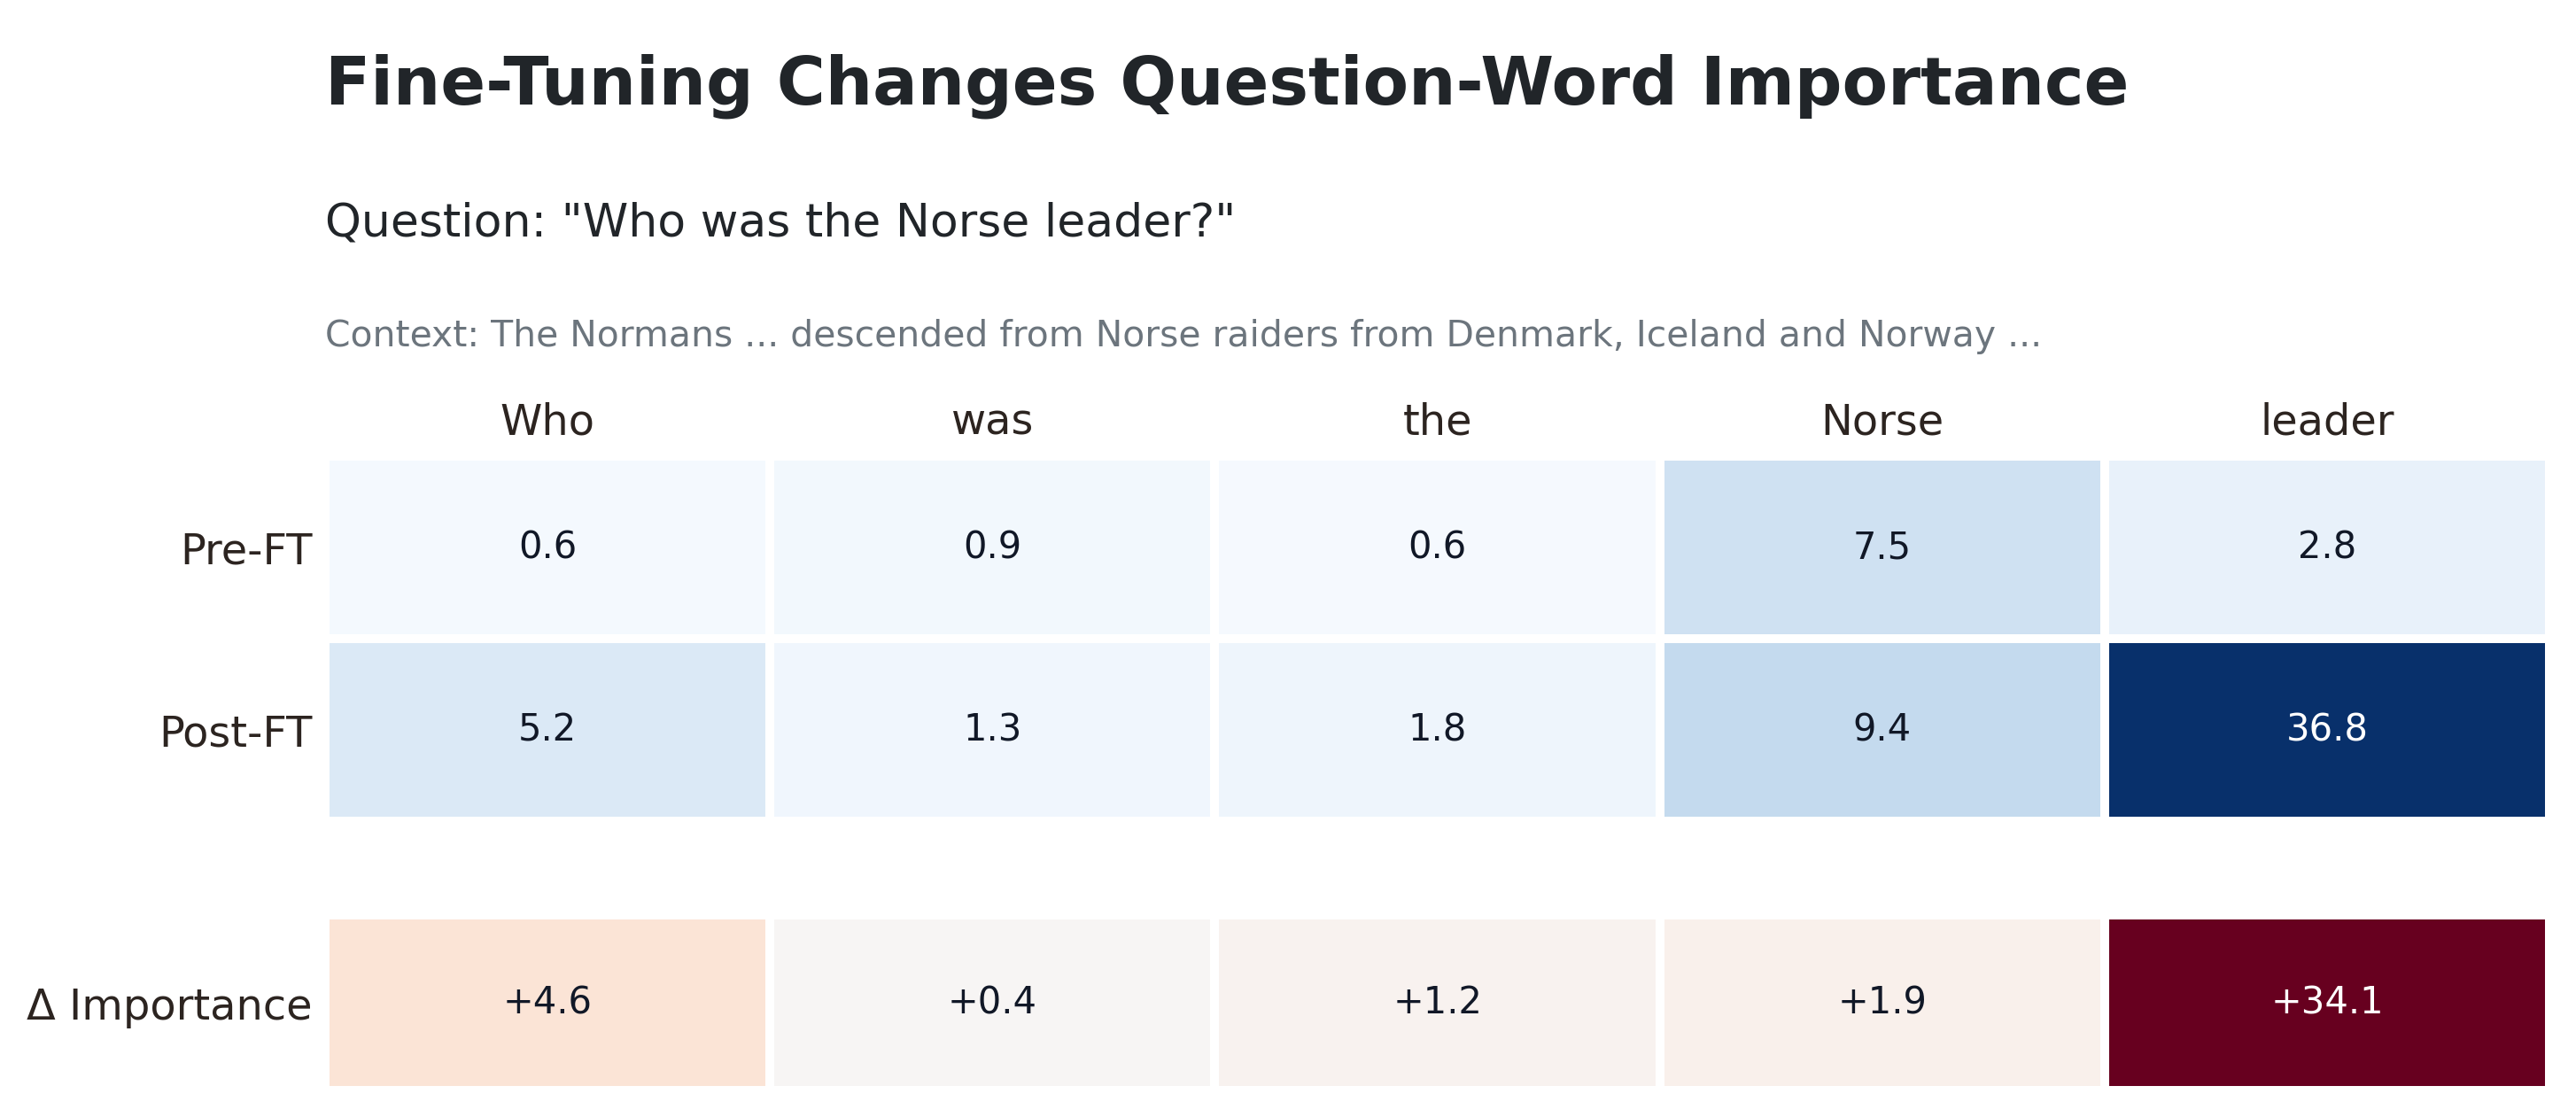
\includegraphics[width=\linewidth]{aiaa4051/task2/comparison/poster_sample3.png}
  \caption{Pre-FT, Post-FT, and Delta CP-LRP heatmaps for a representative
    SQuAD\_v2 sample.
    Blue intensity = absolute relevance magnitude (Blues colormap, Pre-FT and Post-FT rows);
    red/blue diverging colormap (Delta row).
    Post-FT attribution shows stronger emphasis on question-side tokens and
    reduced relevance on uninformative context.}
  \label{fig:task2_comparison}
\end{figure}

\subsection{Aggregate Analysis}

Figure~\ref{fig:mean_delta} shows the mean relevance delta across all 20
samples for each token position.
The bar chart reveals a systematic, position-dependent pattern: token positions
corresponding to the \texttt{Question:} section and the answer-boundary region
show the largest positive mean deltas, while positions in the middle of the
context tend to show near-zero or slightly negative deltas.

To quantify this shift, we partition each sample's tokens into two segments
(the \texttt{Context} field and the \texttt{Question} field) and compute the
mean $\Delta R$ per segment averaged across all 20 samples.
The results confirm the qualitative observation: the \texttt{Question} segment
gains substantially more relevance post fine-tuning
($\overline{\Delta R}_{\text{question}} = +1.67$) compared with the
\texttt{Context} segment ($\overline{\Delta R}_{\text{context}} = +0.27$),
a ratio of approximately $6\times$.
The disproportionate gain on the question side indicates that the fine-tuned
model has learned to weight interrogative structure and content nouns in the
question more heavily when forming its next-token prediction.
Note that positive mean relevance shifts reflect changes in attribution
structure, not necessarily an increase in output confidence; the two should
not be conflated without separate probability-based measurements.

This suggests that the relevance redistribution observed in individual samples
is not idiosyncratic but reflects a consistent shift in the model's internal
attribution strategy following task-specific training.

\subsection{Sequential Fine-Tuning Order}

We chose to fine-tune first on SQuAD\_v2 and then on SciQ based on task
complexity considerations: SQuAD\_v2's long-context reading-comprehension
format is more demanding than SciQ's short, context-free questions, so
beginning with the harder task was expected to establish a broader
contextual processing prior.
The consistently positive mean delta on the \texttt{Question} segment,
without a corresponding regression on context-side relevance, is consistent
with this ordering preserving long-form contextual processing while
adapting to the new answer format.
Whether this ordering was optimal, and whether reversing it
(SciQ$\to$SQuAD) would cause greater catastrophic
interference~\cite{mccloskey1989catastrophic}, can only be established with
a controlled reverse-order ablation, which we leave for future work.

\begin{figure}[t]
  \centering
  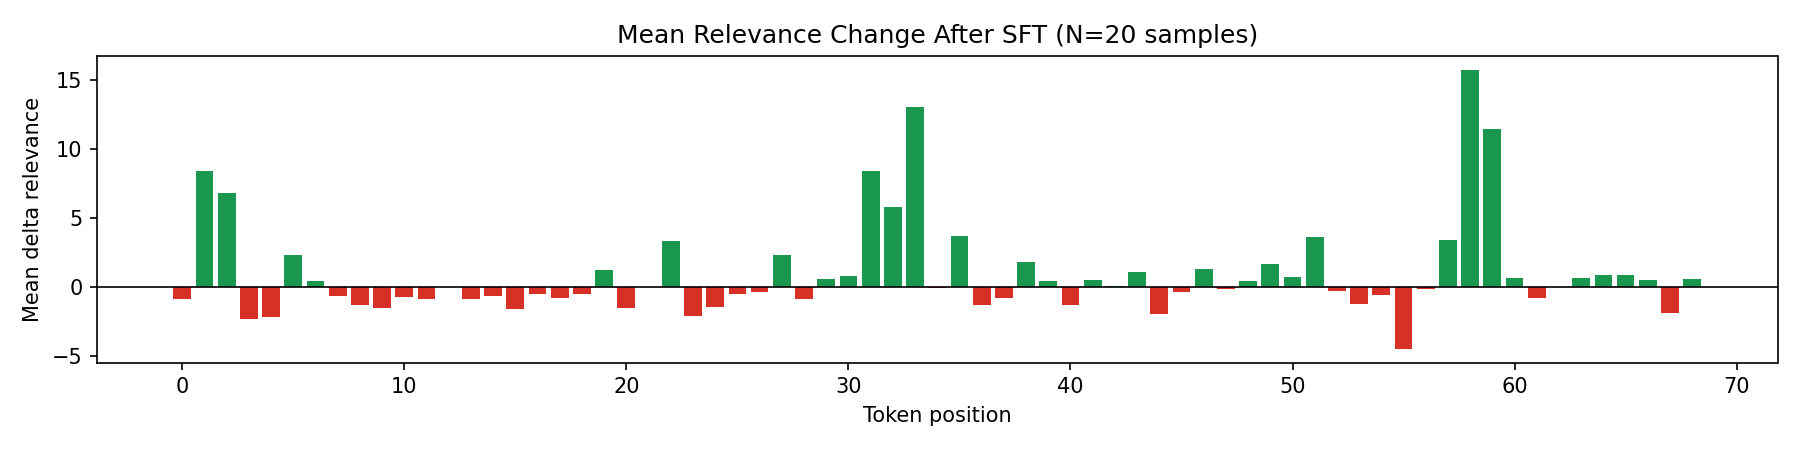
\includegraphics[width=\linewidth]{aiaa4051/task2/comparison/mean_delta.png}
  \caption{Mean relevance delta ($\Delta R = R^{\text{post}} - R^{\text{pre}}$)
    per token position, averaged over $N=20$ SQuAD\_v2 samples.
    Green bars: post-FT assigns more relevance.
    Red bars: post-FT assigns less relevance.}
  \label{fig:mean_delta}
\end{figure}

% ===== SECTION 6: TASK 3 =================
\section{Task 3: Parameter-Level Relevance Comparison}
\label{sec:task3}

\subsection{Experimental Setup}

We train two independent models from the pretrained GPT-2 Small initialisation:

\textbf{Model~A (SciQ):} 3{,}000 SciQ training samples, 3 epochs.
Final training loss: \textbf{0.5227}.

\textbf{Model~B (SQuAD\_v2):} 3{,}000 SQuAD\_v2 training samples, 3 epochs.
Final training loss: \textbf{0.6386}.

For each model, we compute parameter-level relevance via
Equation~\eqref{eq:param-relevance} and normalise by the total across all
12 layers.
Model~A is evaluated on the full SciQ \emph{test} split (1{,}000 samples),
formatted as bare \texttt{Question:\textbackslash nAnswer:} prompts.
Model~B is evaluated on the first 1{,}000 examples of the SQuAD\_v2
\emph{validation} split, formatted with a 300-character context prefix.
Per-layer scores are averaged over all 1{,}000 inputs per model.

\subsection{Results}

Figure~\ref{fig:task3} shows the normalised relevance profiles for both models
alongside their difference ($\Delta = R_A - R_B$; negative values indicate
Model~B relies more on a given layer).
Table~\ref{tab:task3} lists the three layers with the largest absolute
differences.

\begin{table}[h]
  \centering
  \small
  \begin{tabular}{ccl}
    \toprule
    \textbf{Layer} & $\boldsymbol{\Delta}$ \textbf{(A$-$B)} & \textbf{Interpretation} \\
    \midrule
    10 & $+0.0196$ & Model A (SciQ) relies more \\
     9 & $+0.0130$ & Model A (SciQ) relies more \\
     6 & $-0.0126$ & Model B (SQuAD\_v2) relies more \\
    \bottomrule
  \end{tabular}
  \caption{Top-3 layers by absolute normalised relevance difference
    ($\Delta = R_A^{\text{norm}} - R_B^{\text{norm}}$).
    Negative $\Delta$ means Model B engages the layer more strongly.}
  \label{tab:task3}
\end{table}

\begin{figure}[t]
  \centering
  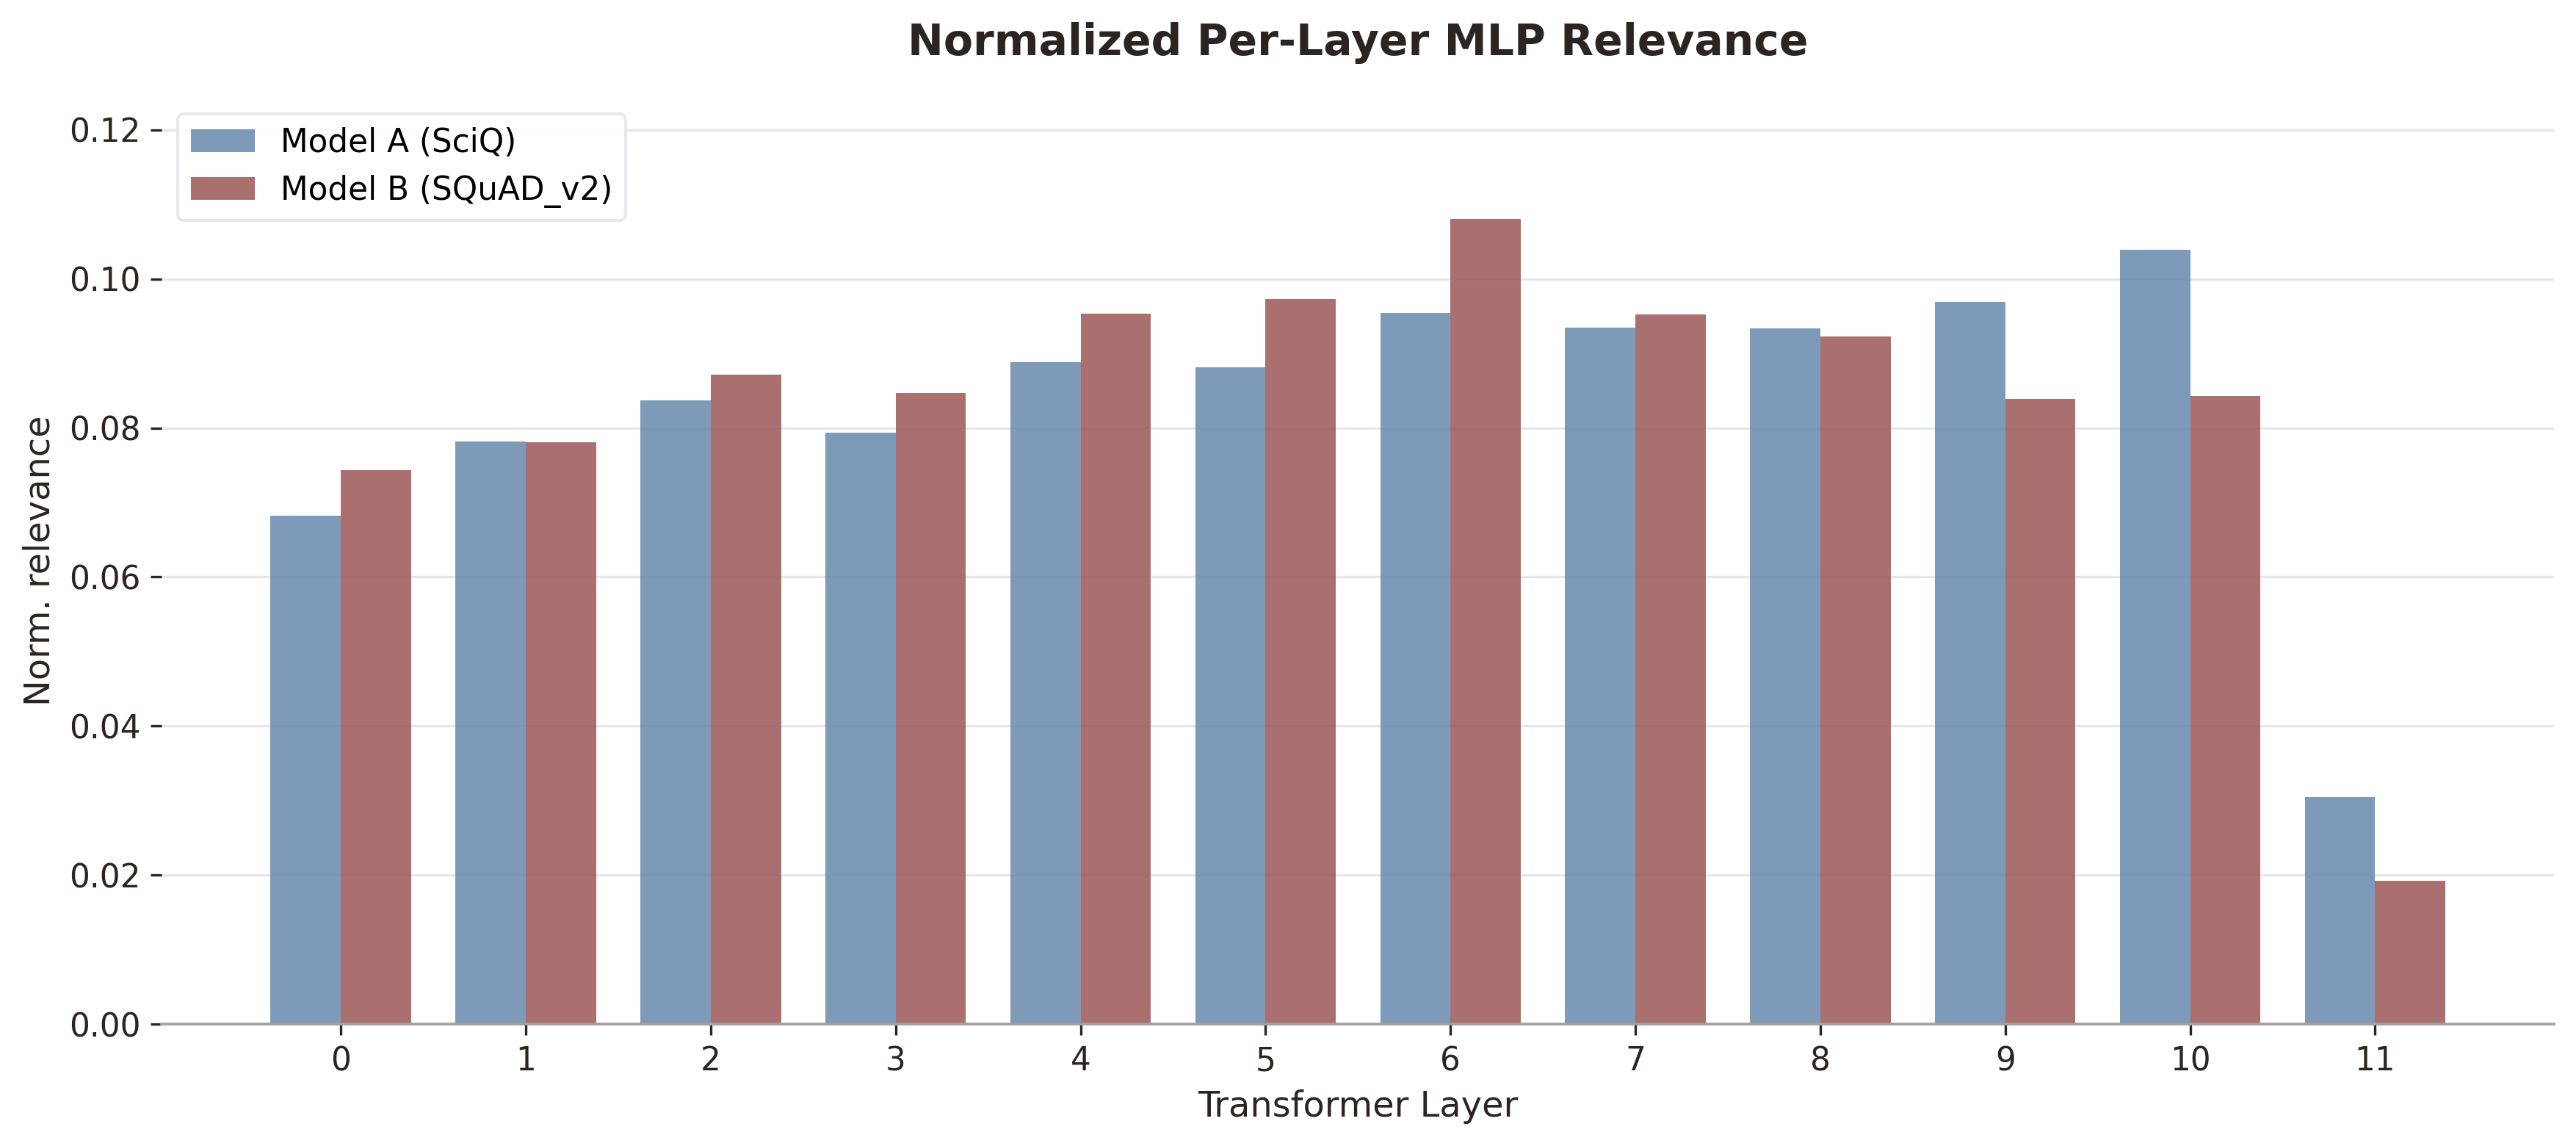
\includegraphics[width=\linewidth]{aiaa4051/task3/comparison/task3_normalized_relevance.png}
  \caption{Normalised per-layer MLP parameter relevance for Model~A (SciQ,
    blue) and Model~B (SQuAD\_v2, red), averaged over 1{,}000 evaluation inputs
    each.
    Model~A peaks at Layer~10 while Model~B concentrates relevance at middle
    layers (Layer~6); see Table~\ref{tab:task3} for numerical differences.}
  \label{fig:task3}
\end{figure}

\subsection{Discussion}

The two models clearly exhibit different layer-relevance profiles despite
sharing the same GPT-2 pretraining initialisation.
Model~A (SciQ) shows a broadly increasing trend in layer engagement from
Layer~0 through Layer~10 ($R^{\text{norm}} = 0.1039$), with a sharp drop at
the final Layer~11 ($R^{\text{norm}} = 0.0305$).
Model~B (SQuAD\_v2) concentrates more relevance in the middle layers,
peaking at Layer~6 ($R^{\text{norm}} = 0.1081$), before declining toward the
upper layers.

The largest absolute differences are at \textbf{Layer~10}
($\Delta = +0.0196$, SciQ higher) and \textbf{Layer~6}
($\Delta = -0.0126$, SQuAD\_v2 higher).
This pattern is consistent with the two tasks' different reliance on
information sources.
SciQ presents questions without any supporting context, so the model must
retrieve answers from its parametric knowledge.
Geva et al.~\cite{geva2021ffn} showed that upper-layer FFN matrices in
transformers function as key-value memories that store factual associations
and project them into the output vocabulary.
The elevated upper-layer engagement in Model~A is therefore consistent with
a heavier reliance on stored parametric knowledge to generate answers.

By contrast, each SQuAD\_v2 prompt always includes a context passage
regardless of answerability: even for the approximately half of SQuAD\_v2
examples that are unanswerable, the model must evaluate the passage to
determine that no answer span is present.
This context-processing demand is absent in SciQ's context-free format,
and it requires integrating positional and semantic information across a
longer input, which is typically handled by intermediate attention and MLP
layers~\cite{geva2021ffn}.
The elevated middle-layer engagement in Model~B at Layer~6 is therefore
consistent with this increased demand for context processing, regardless
of whether a valid answer span exists.

Given that the parameter-level analysis uses 1{,}000 inputs per model drawn
from each model's own training domain (SciQ test set and SQuAD\_v2
validation set), and that the two evaluation sets differ in prompt format
and length (SciQ: short, context-free prompts; SQuAD\_v2: longer,
context-bearing prompts), the observed layer-relevance differences are
confounded by both fine-tuning domain and evaluation input characteristics.
The results should therefore be treated as preliminary evidence consistent
with the proposed parametric-memory vs.\ in-context-retrieval interpretation,
rather than definitive causal effects of fine-tuning domain alone.

% ===== SECTION 7: LIMITATIONS =================
\section{Limitations}
\label{sec:limitations}

\paragraph{Token deletion via attention mask.}
The Pixel Flipping protocol masks tokens by setting \texttt{attention\_mask~=~0}
while leaving token identities and positions unchanged.
This avoids inserting out-of-vocabulary mask tokens into GPT-2's input
stream, but it is not equivalent to literal token deletion: the token
embedding still occupies its original position, and the model observes an
attention pattern that is unlikely to have appeared during pretraining.
Confidence changes under this protocol therefore conflate the attribution
effect with a mild distribution-shift artefact caused by the unusual
masking pattern.
A complementary approach would be to replace masked tokens with a learned
\texttt{[MASK]} embedding or a sampled marginal, which we leave for future
evaluation.

\paragraph{Model scope.}
All experiments are conducted on GPT-2 Small (124M parameters).
Although the CP-LRP patching strategy is in principle applicable to any
GPT-style autoregressive transformer, the attribution patterns and
layer-relevance profiles reported here are specific to this architecture
and scale.
Larger models (e.g., GPT-2 Medium/Large, GPT-J, LLaMA) may exhibit
qualitatively different relevance distributions owing to their greater
depth, wider hidden dimensions, and exposure to more diverse pretraining
data.
Extending this analysis to other model families remains future work.

\paragraph{Parameter-level analysis restricted to MLP weights.}
The parameter-level relevance in Task~3 is computed exclusively over the
two MLP projection matrices (\texttt{c\_fc} and \texttt{c\_proj}) in each
transformer block.
Attention weight matrices (query, key, value, and output projections) are
excluded because enabling gradients on those parameters simultaneously with
the CP-LRP stop-gradient patches on the query and key activations would
create an inconsistency in the backward graph.
Consequently, the reported layer profiles reflect only the MLP contribution
to parameter-level relevance; a complete picture would require an extended
formulation that handles attention weight gradients under CP-LRP constraints.

\paragraph{Small evaluation sample for Task~2.}
Task~2 compares attributions on 20 SQuAD\_v2 samples, so the quantitative
segment-level estimates (e.g., mean $\Delta R$ per segment) carry substantial
variance.
Larger evaluation sets, covering a more diverse range of question types and
context lengths, would strengthen the statistical reliability of the
observed relevance shifts.

% ===== SECTION 8: CONCLUSION =================
\section{Conclusion}
\label{sec:conclusion}

We have applied CP-LRP (AttnLRP) to GPT-2 Small across three levels of
analysis, with the following findings:

\textbf{Token level (Task~1):} CP-LRP reliably assigns the highest positive
relevance to named entities and question keywords in a QA context.
Pixel Flipping confirms attribution faithfulness: the AttnLRP AUC (0.0190) is
substantially lower than the random baseline (0.0490) and the
least-relevant-first baseline (0.0871), providing perturbation-based evidence that CP-LRP scores rank tokens
in a way consistent with their causal influence on next-token confidence.
The AttnLRP curve is non-monotonic: confidence partially recovers at
60\% to 70\% masking when negatively-relevant (suppressive) tokens begin to be
removed, motivating supplementary polarity-aware metrics such as
comprehensiveness and sufficiency for signed attribution methods.

\textbf{Fine-tuning effects (Task~2):} Sequential fine-tuning on SQuAD\_v2
followed by SciQ systematically shifts CP-LRP attributions toward
question-side tokens and answer-relevant entities, while de-emphasising
mid-context background information.
AttnLRP can thus serve as a diagnostic tool for detecting the behavioural
fingerprint of task-specific training.

\textbf{Parameter level (Task~3):} Evaluated over 1{,}000 inputs each,
the SciQ-finetuned model shows higher engagement at upper MLP layers
(peak at Layer~10, $\Delta = +0.0196$), while the SQuAD\_v2-finetuned model
concentrates more relevance in middle layers (peak at Layer~6,
$\Delta = -0.0126$).
This is consistent with SciQ requiring parametric memory recall from upper
FFN layers, whereas SQuAD\_v2's longer context-bearing prompts require more
middle-layer context processing.

These results suggest that AttnLRP, implemented via the CP-LRP variant, is a
practical and informative framework for auditing attribution patterns in
autoregressive language models at multiple granularities.

Several directions remain for future work.
First, extending the three-level analysis to larger autoregressive models
(e.g., GPT-2 Medium/Large, LLaMA) would test whether the layer-relevance
profiles and fine-tuning signatures observed here are specific to GPT-2 Small
or reflect more general properties of transformer-based LMs.
Second, replacing the signed-relevance ordering in the Pixel Flipping
protocol with an absolute-magnitude ordering, and incorporating
polarity-aware metrics such as comprehensiveness and sufficiency, would
provide a more complete faithfulness evaluation for signed attribution methods.
Third, expanding the parameter-level analysis to include attention weight
matrices (requiring an extended CP-LRP formulation that handles stop-gradient
constraints on Q/K projections) would give a fuller picture of how fine-tuning
redistributes relevance across all learnable parameters, not only the MLP
components.

% ===== CONTRIBUTIONS =================
\section*{Author Contributions}

\textbf{Yenchi Tseng} implemented and ran the Task~1 token attribution
experiments and the Task~3 parameter-level relevance analysis, designed and
produced the project poster, and contributed to report writing.
\textbf{Fangteng Fu} implemented and ran the Task~2 sequential fine-tuning
experiments and the Task~3 parameter-level relevance analysis, and contributed
to report writing.
The report was jointly written by both authors.

% ===== REFERENCES =================
\begin{thebibliography}{99}

\bibitem{achtibat2024attnlrp}
R.~Achtibat, S.\,M.\,V.~Hatefi, M.~Dreyer, A.~Jain, T.~Wiegand,
S.~Lapuschkin, and W.~Samek.
\newblock AttnLRP: Attention-aware layer-wise relevance propagation for
  transformers.
\newblock In \emph{Proceedings of the 41st International Conference on Machine
  Learning (ICML)}, 2024.

\bibitem{bach2015pixel}
S.~Bach, A.~Binder, G.~Montavon, F.~Klauschen, K.-R.~M{\"u}ller, and
W.~Samek.
\newblock On pixel-wise explanations for non-linear classifier decisions by
  layer-wise relevance propagation.
\newblock \emph{PLOS ONE}, 10(7):e0130140, 2015.

\bibitem{radford2019gpt2}
A.~Radford, J.~Wu, R.~Child, D.~Luan, D.~Amodei, and I.~Sutskever.
\newblock Language models are unsupervised multitask learners.
\newblock \emph{OpenAI Blog}, 1(8):9, 2019.

\bibitem{rajpurkar2018squad2}
P.~Rajpurkar, R.~Jia, and P.~Liang.
\newblock Know what you don't know: Unanswerable questions for SQuAD.
\newblock In \emph{Proceedings of the 56th Annual Meeting of the Association
  for Computational Linguistics (ACL)}, pages 784--789, 2018.

\bibitem{welbl2017sciq}
J.~Welbl, N.\,F.~Liu, and M.~Gardner.
\newblock Crowdsourcing multiple choice science questions.
\newblock In \emph{Proceedings of the 3rd Workshop on Noisy User-generated
  Text}, pages 94--106, 2017.

\bibitem{samek2017evaluating}
W.~Samek, A.~Binder, G.~Montavon, S.~Lapuschkin, and K.-R.~M{\"u}ller.
\newblock Evaluating the visualization of what a deep neural network has
  learned.
\newblock \emph{IEEE Transactions on Neural Networks and Learning Systems},
  28(11):2660--2673, 2017.

\bibitem{jain2019attention}
S.~Jain and B.~C.~Wallace.
\newblock Attention is not explanation.
\newblock In \emph{Proceedings of the 2019 Conference of the North American
  Chapter of the Association for Computational Linguistics (NAACL)},
  pages 3543--3556, 2019.

\bibitem{wiegreffe2019attention}
S.~Wiegreffe and Y.~Pinter.
\newblock Attention is not not explanation.
\newblock In \emph{Proceedings of the 2019 Conference on Empirical Methods
  in Natural Language Processing (EMNLP)}, pages 11--20, 2019.

\bibitem{geva2021ffn}
M.~Geva, R.~Schuster, J.~Berant, and O.~Levy.
\newblock Transformer feed-forward layers are key-value memories.
\newblock In \emph{Proceedings of the 2021 Conference on Empirical Methods
  in Natural Language Processing (EMNLP)}, pages 5484--5495, 2021.

\bibitem{mccloskey1989catastrophic}
M.~McCloskey and N.~J.~Cohen.
\newblock Catastrophic interference in connectionist networks: The sequential
  learning problem.
\newblock \emph{Psychology of Learning and Motivation}, 24:109--165, 1989.

\end{thebibliography}

\end{document}
